\pgfdeclarelayer{edgelayer}
\pgfdeclarelayer{nodelayer}
\pgfsetlayers{edgelayer,nodelayer,main}



\tikzset{->-/.style={decoration={
  markings,
  mark=at position .5 with {\arrow{>}}},postaction={decorate}}}

\tikzstyle{none}=[inner sep=0pt]
\tikzstyle{contact}=[circle, fill=black, draw, inner sep=1.5pt, anchor=center]
\tikzstyle{bdot}=[circle, fill=black, draw, inner sep=1.5pt, anchor=center]
\tikzstyle{wdot}=[circle, fill=white, draw, inner sep=1.5pt]
\tikzstyle{bwdot}=[circle, fill=white, draw, inner sep=3pt]
\tikzstyle{bamp}=[rounded rectangle, rounded rectangle west arc=0pt, draw, inner
sep = 2pt,minimum width=4ex,minimum height=2ex,fill=black,text=white]
\tikzstyle{bampop}=[rounded rectangle, rounded rectangle east arc=0pt, draw, inner
sep = 2pt,minimum width=4ex,minimum height=2ex,fill=black,text=white]
\tikzstyle{wamp}=[rounded rectangle, rounded rectangle west arc=0pt, draw, inner
sep = 2pt,minimum width=4ex,minimum height=2ex,fill=white]
\tikzstyle{wampop}=[rounded rectangle, rounded rectangle east arc=0pt, draw, inner
sep = 2pt,minimum width=4ex,minimum height=2ex,fill=white]



  \tikzset{
     tick/.style={postaction={
        decorate,
        decoration={markings, mark=at position 0.5 with
        {\draw[-] (0,.4ex) -- (0,-.4ex);}}}
     }
  } 
  
  \tikzset{
     functor/.style={->, thick, shorten <=4pt, shorten >=4pt}
  }

  \tikzset{
     function/.style={->, thin, shorten <=4pt, shorten >=4pt}
  }

  \tikzset{
     mapsto/.style={->, densely dashed, blue, shorten <=\short, shorten
     >=\short, >=stealth, thick},
     short/.store in=\short,
     short=0pt
  }
  
\tikzset{
	spider diagram/.style={
		every to/.style={out=0, in=180, draw, thick},
		thick
	},
	dot size/.store in=\dotsize,
	dot size = 5pt,
	leg length/.store in=\leglen,
	leg length = 15pt,
	baby/.style={dot size = 2pt, leg length = 6pt},
	young/.style={dot size = 3pt, leg length = 10pt},
	special spider/.code n args={4}{
		\pgfkeysalso{circle, draw, thick, inner sep=0, minimum width=\dotsize,
  		prefix after command={\pgfextra{\let\fixname\tikzlastnode}},
  		append after command={\pgfextra{
  			\ifnum #1=0{} \else {\foreach \i in {1,...,#1} {
					\tikzmath{\anglei={-90*(#1+1-2*\i)/#1};}
  				\draw [thick]
						(\fixname) .. controls 
						($(\fixname.center)-(\anglei:#3/3)$) and ($(\fixname.center)-(\anglei:#3*2/3)$) .. 
						({$(\fixname)-(\anglei:#3*2/3)$}-|{$(\fixname)-(#3,0)$}) coordinate (\fixname_in\i);
  			}}\fi
  			\ifnum #2=0{} \else {\foreach \i in {1,...,#2} {
					\tikzmath{\anglei={90*(#2+1-2*\i)/#2};}
  				\draw [thick]
						(\fixname.center) .. controls 
						($(\fixname.center)+(\anglei:#4/3)$) and ($(\fixname.center)+(\anglei:#4*2/3)$) .. 
						({$(\fixname.center)+(\anglei:#4*2/3)$}-|{$(\fixname.center)+(#4,0)$}) coordinate (\fixname_out\i);
  			}}\fi
  		}}
		}
	},
	spider/.code 2 args={
		\pgfkeysalso{special spider={#1}{#2}{\leglen}{\leglen}}
	}
}


  	
  \tikzset{
     oriented WD/.style={%everything after equals replaces "oriented WD" in key.
        every to/.style={out=0,in=180,draw},
        label/.style={
           font=\everymath\expandafter{\the\everymath\scriptstyle},
           inner sep=0pt,
           node distance=2pt and -2pt},
        semithick,
        node distance=1 and 1,
        decoration={markings, mark=at position \stringdecpos with \stringdec},
        ar/.style={postaction={decorate}},
        execute at begin picture={\tikzset{
           x=\bbx, y=\bby,
           every fit/.style={inner xsep=\bbx, inner ysep=\bby}}}
        },
     string decoration/.store in=\stringdec,
     string decoration={\arrow{stealth};},
     string decoration pos/.store in=\stringdecpos,
     string decoration pos=.7,
     bbx/.store in=\bbx,
     bbx = 1.5cm,
     bby/.store in=\bby,
     bby = 1.5ex,
     bb port sep/.store in=\bbportsep,
     bb port sep=1.5,
     % bb wire sep/.store in=\bbwiresep,
     % bb wire sep=1.75ex,
     bb port length/.store in=\bbportlen,
     bb port length=4pt,
     bb penetrate/.store in=\bbpenetrate,
     bb penetrate=0,
     bb min width/.store in=\bbminwidth,
     bb min width=1cm,
     bb rounded corners/.store in=\bbcorners,
     bb rounded corners=2pt,
     bb small/.style={bb port sep=1, bb port length=2.5pt, bbx=.4cm, bb min width=.4cm, 
bby=.7ex},
		 bb medium/.style={bb port sep=1, bb port length=2.5pt, bbx=.4cm, bb min width=.4cm, 
bby=.9ex},
     bb/.code 2 args={%When you see this key, run the code below:
        \pgfmathsetlengthmacro{\bbheight}{\bbportsep * (max(#1,#2)+1) * \bby}
        \pgfkeysalso{draw,minimum height=\bbheight,minimum width=\bbminwidth,outer 
sep=0pt,
           rounded corners=\bbcorners,thick,
           prefix after command={\pgfextra{\let\fixname\tikzlastnode}},
           append after command={\pgfextra{\draw
              \ifnum #1=0{} \else foreach \i in {1,...,#1} {
                 ($(\fixname.north west)!{\i/(#1+1)}!(\fixname.south west)$) +(-
\bbportlen,0) 
  coordinate (\fixname_in\i) -- +(\bbpenetrate,0) coordinate (\fixname_in\i')}\fi 
  %Define the endpoints of tickmarks
              \ifnum #2=0{} \else foreach \i in {1,...,#2} {
                 ($(\fixname.north east)!{\i/(#2+1)}!(\fixname.south east)$) +(-
\bbpenetrate,0) 
  coordinate (\fixname_out\i') -- +(\bbportlen,0) coordinate (\fixname_out\i)}\fi;
           }}}
     },
     bb name/.style={append after command={\pgfextra{\node[anchor=north] at 
(\fixname.north) {#1};}}}
  }
  
  
  \tikzset{
  	unoriented WD/.style={
  		every to/.style={draw},
  		shorten <=-\penetration, shorten >=-\penetration,
  		label distance=-2pt,
  		thick,
  		node distance=\spacing,
  		execute at begin picture={\tikzset{
  			x=\spacing, y=\spacing}}
  		},
  	pack size/.store in=\psize,
  	pack size = 8pt,
  	spacing/.store in=\spacing,
  	spacing = 8pt,
  	link size/.store in=\lsize,
  	link size = 2pt,
		penetration/.store in=\penetration,
		penetration = 2pt,
  	pack color/.store in=\pcolor,
  	pack color = blue,
  	pack inside color/.store in=\picolor,
  	pack inside color=blue!20,
  	pack outside color/.store in=\pocolor,
  	pack outside color=blue!50!black,
  	surround sep/.store in=\ssep,
  	surround sep=8pt,
  	link/.style={
  		circle, 
  		draw=black, 
  		fill=black,
  		inner sep=0pt, 
  		minimum size=\lsize
  	},
  	pack/.style={
  		circle, 
  		draw = \pocolor, 
  		fill = \picolor,
  		inner sep = .25*\psize,
  		minimum size = \psize
  	},
  	outer pack/.style={
  		ellipse, 
  		draw,
  		inner sep=\ssep,
  		color=\pocolor,
  	},
  	intermediate pack/.style={
  		ellipse,
  		dashed, 
  		draw,
  		inner sep=\ssep,
  		color=\pocolor,
  	},
  }

	\tikzcdset{
		bijection/.style={every arrow/.append style={dash}}
	}
	
	
\newcommand{\scalar}[1]
{
\begin{aligned}
    \resizebox{#1}{!}{
\begin{tikzpicture}
	\begin{pgfonlayer}{nodelayer}
		\node [style=none] (0) at (-.75, 0) {};
		\node [style=wamp] (1) at (0, 0) {$a$};
		\node [style=none] (2) at (.75, 0) {};
	\end{pgfonlayer}
	\begin{pgfonlayer}{edgelayer}
		\draw[line width=1.25pt] (0.center) to (1.center);
		\draw[line width=1.25pt] (1.center) to (2.center);
	\end{pgfonlayer}
      \end{tikzpicture}}
\end{aligned}
}
	
\newcommand{\mult}[1]
{
\begin{aligned}
    \resizebox{#1}{!}{
\begin{tikzpicture}
	\begin{pgfonlayer}{nodelayer}
		\node [style=none] (0) at (1, -0) {};
		\node [style=circ] (1) at (0.125, -0) {};
		\node [style=none] (2) at (-1, 0.5) {};
		\node [style=none] (3) at (-1, -0.5) {};
	\end{pgfonlayer}
	\begin{pgfonlayer}{edgelayer}
		\draw[line width=2pt] (0.center) to (1.center);
		\draw[line width=2pt] [in=0, out=120, looseness=1.20] (1.center) to (2.center);
		\draw[line width=2pt] [in=0, out=-120, looseness=1.20] (1.center) to (3.center);
	\end{pgfonlayer}
      \end{tikzpicture}}
\end{aligned}
}

\newcommand{\add}[1]
{
\begin{aligned}
    \resizebox{#1}{!}{
\begin{tikzpicture}
	\begin{pgfonlayer}{nodelayer}
		\node [style=none] (0) at (1, -0) {};
		\node [style=circw] (1) at (0.125, -0) {};
		\node [style=none] (2) at (-1, 0.5) {};
		\node [style=none] (3) at (-1, -0.5) {};
	\end{pgfonlayer}
	\begin{pgfonlayer}{edgelayer}
		\draw[line width=2pt] (0.center) to (1.center);
		\draw[line width=2pt] [in=0, out=120, looseness=1.20] (1.center) to (2.center);
		\draw[line width=2pt] [in=0, out=-120, looseness=1.20] (1.center) to (3.center);
	\end{pgfonlayer}
      \end{tikzpicture}}
\end{aligned}
}

\newcommand{\unit}[1]
{
  \begin{aligned}
    \resizebox{#1}{!}{
\begin{tikzpicture}
	\begin{pgfonlayer}{nodelayer}
		\node [style=none] (spaceup) at (0, 0.5) {};
		\node [style=none] (spacedown) at (0, -0.5) {};
		\node [style=none] (0) at (1, -0) {};
		\node [style=none] (1) at (-1, -0) {};
		\node [style=circ] (2) at (0, -0) {};
	\end{pgfonlayer}
	\begin{pgfonlayer}{edgelayer}
		\draw[line width=2pt] (0.center) to (2);
	\end{pgfonlayer}
      \end{tikzpicture}}
  \end{aligned}
}

\newcommand{\zero}[1]
{
  \begin{aligned}
    \resizebox{#1}{!}{
\begin{tikzpicture}
	\begin{pgfonlayer}{nodelayer}
		\node [style=none] (spaceup) at (0, 0.5) {};
		\node [style=none] (spacedown) at (0, -0.5) {};
		\node [style=none] (0) at (1, -0) {};
		\node [style=none] (1) at (-1, -0) {};
		\node [style=circw] (2) at (0, -0) {};
	\end{pgfonlayer}
	\begin{pgfonlayer}{edgelayer}
		\draw[line width=2pt] (0.center) to (2);
	\end{pgfonlayer}
      \end{tikzpicture}}
  \end{aligned}
}

\newcommand{\comult}[1]
{
\begin{aligned}
    \resizebox{#1}{!}{
\begin{tikzpicture}
	\begin{pgfonlayer}{nodelayer}
		\node [style=none] (0) at (-1, -0) {};
		\node [style=circ] (1) at (-0.125, -0) {};
		\node [style=none] (2) at (1, 0.5) {};
		\node [style=none] (3) at (1, -0.5) {};
	\end{pgfonlayer}
	\begin{pgfonlayer}{edgelayer}
		\draw[line width=2pt] (0.center) to (1.center);
		\draw[line width=2pt] [in=180, out=60, looseness=1.20] (1.center) to (2.center);
		\draw[line width=2pt] [in=180, out=-60, looseness=1.20] (1.center) to (3.center);
	\end{pgfonlayer}
      \end{tikzpicture}}
\end{aligned}
}

\newcommand{\counit}[1]
{
  \begin{aligned}
    \resizebox{#1}{!}{
\begin{tikzpicture}
	\begin{pgfonlayer}{nodelayer}
		\node [style=none] (spaceup) at (0, 0.5) {};
		\node [style=none] (spacedown) at (0, -0.5) {};
		\node [style=none] (0) at (-1, -0) {};
		\node [style=none] (1) at (1, -0) {};
		\node [style=circ] (2) at (0, -0) {};
	\end{pgfonlayer}
	\begin{pgfonlayer}{edgelayer}
		\draw[line width=2pt] (0.center) to (2);
	\end{pgfonlayer}
      \end{tikzpicture}}
  \end{aligned}
}

\newcommand{\coadd}[1]
{
\begin{aligned}
    \resizebox{#1}{!}{
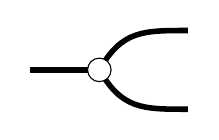
\begin{tikzpicture}
	\begin{pgfonlayer}{nodelayer}
		\node [style=none] (0) at (-1, -0) {};
		\node [style=bwdot] (1) at (-0.125, -0) {};
		\node [style=none] (2) at (1, 0.5) {};
		\node [style=none] (3) at (1, -0.5) {};
	\end{pgfonlayer}
	\begin{pgfonlayer}{edgelayer}
		\draw[line width=2pt] (0.center) to (1.center);
		\draw[line width=2pt] [in=180, out=60, looseness=1.20] (1.center) to (2.center);
		\draw[line width=2pt] [in=180, out=-60, looseness=1.20] (1.center) to (3.center);
	\end{pgfonlayer}
      \end{tikzpicture}}
\end{aligned}
}

\newcommand{\cozero}[1]
{
  \begin{aligned}
    \resizebox{#1}{!}{
\begin{tikzpicture}
	\begin{pgfonlayer}{nodelayer}
		\node [style=none] (spaceup) at (0, 0.5) {};
		\node [style=none] (spacedown) at (0, -0.5) {};
		\node [style=none] (0) at (-1, -0) {};
		\node [style=none] (1) at (1, -0) {};
		\node [style=bwdot] (2) at (0, -0) {};
	\end{pgfonlayer}
	\begin{pgfonlayer}{edgelayer}
		\draw[line width=2pt] (0.center) to (2);
	\end{pgfonlayer}
      \end{tikzpicture}}
  \end{aligned}
}

\newcommand{\idone}[1]
{
  \begin{aligned}
    \resizebox{#1}{!}{
     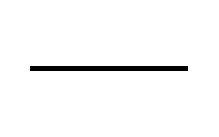
\begin{tikzpicture}
	\begin{pgfonlayer}{nodelayer}
		\node [style=none] (0) at (-1, -0) {};
		\node [style=none] (1) at (1, -0) {};
		\node [style=none] (2) at (0, 0.5) {};
		\node [style=none] (3) at (0, -0.5) {};
	\end{pgfonlayer}
	\begin{pgfonlayer}{edgelayer}
		\draw[line width=2pt] (1.center) to (0.center);
	\end{pgfonlayer}
\end{tikzpicture} 
    }
  \end{aligned}
}

\newcommand{\swap}[1]
{
  \begin{aligned}
    \resizebox{#1}{!}{
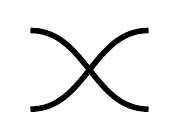
\begin{tikzpicture}
	\begin{pgfonlayer}{nodelayer}
		\node [style=none] (2) at (-0.5, -0.5) {};
		\node [style=none] (3) at (-2, 0.5) {};
		\node [style=none] (4) at (-0.5, 0.5) {};
		\node [style=none] (5) at (-2, -0.5) {};
	\end{pgfonlayer}
	\begin{pgfonlayer}{edgelayer}
		\draw[line width=2pt] [in=180, out=0, looseness=1.00] (3.center) to (2.center);
		\draw[line width=2pt] [in=0, out=180, looseness=1.00] (4.center) to (5.center);
	\end{pgfonlayer}
\end{tikzpicture}
    }
  \end{aligned}
}
%%fakesubsubsection associativity
\newcommand{\assocl}[1]
{
  \begin{aligned}
    \resizebox{#1}{!}{
\begin{tikzpicture}
	\begin{pgfonlayer}{nodelayer}
		\node [style=circ] (0) at (0.125, -0) {};
		\node [style=none] (1) at (-1, 0.5) {};
		\node [style=none] (2) at (-1, -0.5) {};
		\node [style=none] (3) at (0, -1) {};
		\node [style=none] (4) at (2.25, -0.5) {};
		\node [style=none] (5) at (0.25, -0) {};
		\node [style=circ] (6) at (1.25, -0.5) {};
		\node [style=none] (7) at (-1, -1) {};
	\end{pgfonlayer}
	\begin{pgfonlayer}{edgelayer}
		\draw[line width=2pt] [in=0, out=120, looseness=1.20] (0.center) to (1.center);
		\draw[line width=2pt] [in=0, out=-120, looseness=1.20] (0.center) to (2.center);
		\draw[line width=2pt] (4.center) to (6);
		\draw[line width=2pt] [in=0, out=120, looseness=1.20] (6) to (5.center);
		\draw[line width=2pt] [in=0, out=-120, looseness=1.20] (6) to (3.center);
		\draw[line width=2pt] (3.center) to (7.center);
	\end{pgfonlayer}
      \end{tikzpicture}}
  \end{aligned}
}


\newcommand{\assocr}[1]
{
  \begin{aligned}
    \resizebox{#1}{!}{
\begin{tikzpicture}
	\begin{pgfonlayer}{nodelayer}
		\node [style=circ] (0) at (0.125, -0.5) {};
		\node [style=none] (1) at (-1, -1) {};
		\node [style=none] (2) at (-1, 0) {};
		\node [style=none] (3) at (0, 0.5) {};
		\node [style=none] (4) at (2.25, 0) {};
		\node [style=none] (5) at (0.25, -0.5) {};
		\node [style=circ] (6) at (1.25, 0) {};
		\node [style=none] (7) at (-1, 0.5) {};
	\end{pgfonlayer}
	\begin{pgfonlayer}{edgelayer}
		\draw[line width=2pt] [in=0, out=-120, looseness=1.20] (0.center) to (1.center);
		\draw[line width=2pt] [in=0, out=120, looseness=1.20] (0.center) to (2.center);
		\draw[line width=2pt] (4.center) to (6);
		\draw[line width=2pt] [in=0, out=-120, looseness=1.20] (6) to (5.center);
		\draw[line width=2pt] [in=0, out=120, looseness=1.20] (6) to (3.center);
		\draw[line width=2pt] (3.center) to (7.center);
	\end{pgfonlayer}
      \end{tikzpicture}}
  \end{aligned}
}


\newcommand{\coassocl}[1]
{
  \begin{aligned}
    \resizebox{#1}{!}{
\begin{tikzpicture}
	\begin{pgfonlayer}{nodelayer}
		\node [style=circ] (0) at (1.125, -0.5) {};
		\node [style=none] (1) at (2.25, -1) {};
		\node [style=none] (2) at (2.25, 0) {};
		\node [style=none] (3) at (1.25, 0.5) {};
		\node [style=none] (4) at (-1, 0) {};
		\node [style=none] (5) at (1, -0.5) {};
		\node [style=circ] (6) at (0, 0) {};
		\node [style=none] (7) at (2.25, 0.5) {};
	\end{pgfonlayer}
	\begin{pgfonlayer}{edgelayer}
		\draw[line width=2pt] [in=180, out=-60, looseness=1.20] (0.center) to (1.center);
		\draw[line width=2pt] [in=180, out=60, looseness=1.20] (0.center) to (2.center);
		\draw[line width=2pt] (4.center) to (6);
		\draw[line width=2pt] [in=180, out=-60, looseness=1.20] (6) to (5.center);
		\draw[line width=2pt] [in=180, out=60, looseness=1.20] (6) to (3.center);
		\draw[line width=2pt] (3.center) to (7.center);
	\end{pgfonlayer}
      \end{tikzpicture}}
  \end{aligned}
}


\newcommand{\coassocr}[1]
{
  \begin{aligned}
    \resizebox{#1}{!}{
\begin{tikzpicture}
	\begin{pgfonlayer}{nodelayer}
		\node [style=circ] (0) at (1.125, 0) {};
		\node [style=none] (1) at (2.25, 0.5) {};
		\node [style=none] (2) at (2.25, -0.5) {};
		\node [style=none] (3) at (1.25, -1) {};
		\node [style=none] (4) at (-1, -0.5) {};
		\node [style=none] (5) at (1, 0) {};
		\node [style=circ] (6) at (0, -0.5) {};
		\node [style=none] (7) at (2.25, -1) {};
	\end{pgfonlayer}
	\begin{pgfonlayer}{edgelayer}
		\draw[line width=2pt] [in=180, out=60, looseness=1.20] (0.center) to (1.center);
		\draw[line width=2pt] [in=180, out=-60, looseness=1.20] (0.center) to (2.center);
		\draw[line width=2pt] (4.center) to (6);
		\draw[line width=2pt] [in=180, out=60, looseness=1.20] (6) to (5.center);
		\draw[line width=2pt] [in=180, out=-60, looseness=1.20] (6) to (3.center);
		\draw[line width=2pt] (3.center) to (7.center);
	\end{pgfonlayer}
      \end{tikzpicture}}
  \end{aligned}
}

%%fakesubsubsection unitality
\newcommand{\unitl}[1]
{
  \begin{aligned}
    \resizebox{#1}{!}{
\begin{tikzpicture}
	\begin{pgfonlayer}{nodelayer}
		\node [style=none] (0) at (1, -0) {};
		\node [style=circ] (1) at (0.125, -0) {};
		\node [style=circ] (2) at (-1, 0.5) {};
		\node [style=none] (3) at (-1, -0.5) {};
		\node [style=none] (4) at (-2, -0.5) {};
	\end{pgfonlayer}
	\begin{pgfonlayer}{edgelayer}
		\draw[line width=2pt] (0.center) to (1.center);
		\draw[line width=2pt] [in=0, out=120, looseness=1.20] (1.center) to (2.center);
		\draw[line width=2pt] [in=0, out=-120, looseness=1.20] (1.center) to (3.center);
		\draw[line width=2pt] (4.center) to (3.center);
	\end{pgfonlayer}
\end{tikzpicture}
    }
  \end{aligned}
}

\newcommand{\counitl}[1]
{
  \begin{aligned}
    \resizebox{#1}{!}{
\begin{tikzpicture}
	\begin{pgfonlayer}{nodelayer}
		\node [style=none] (0) at (-2, -0) {};
		\node [style=circ] (1) at (-1.125, -0) {};
		\node [style=circ] (2) at (0, 0.5) {};
		\node [style=none] (3) at (0, -0.5) {};
		\node [style=none] (4) at (1, -0.5) {};
	\end{pgfonlayer}
	\begin{pgfonlayer}{edgelayer}
		\draw[line width=2pt] (0.center) to (1.center);
		\draw[line width=2pt] [in=180, out=60, looseness=1.20] (1.center) to (2.center);
		\draw[line width=2pt] [in=180, out=-60, looseness=1.20] (1.center) to (3.center);
		\draw[line width=2pt] (4.center) to (3.center);
	\end{pgfonlayer}
\end{tikzpicture}
    }
  \end{aligned}
}

%%fakesubsubsection commutativity
\newcommand{\commute}[1]
{
  \begin{aligned}
    \resizebox{#1}{!}{
\begin{tikzpicture}
	\begin{pgfonlayer}{nodelayer}
		\node [style=none] (0) at (1.25, -0) {};
		\node [style=circ] (1) at (0.375, -0) {};
		\node [style=none] (2) at (-0.5, -0.5) {};
		\node [style=none] (3) at (-2, 0.5) {};
		\node [style=none] (4) at (-0.5, 0.5) {};
		\node [style=none] (5) at (-2, -0.5) {};
	\end{pgfonlayer}
	\begin{pgfonlayer}{edgelayer}
		\draw[line width=2pt] (0.center) to (1.center);
		\draw[line width=2pt] [in=0, out=-120, looseness=1.20] (1.center) to (2.center);
		\draw[line width=2pt] [in=180, out=0, looseness=1.00] (3.center) to (2.center);
		\draw[line width=2pt] [in=0, out=120, looseness=1.20] (1.center) to (4.center);
		\draw[line width=2pt] [in=0, out=180, looseness=1.00] (4.center) to (5.center);
	\end{pgfonlayer}
\end{tikzpicture}
    }
  \end{aligned}
}


\newcommand{\cocommute}[1]
{
  \begin{aligned}
    \resizebox{#1}{!}{
\begin{tikzpicture}
	\begin{pgfonlayer}{nodelayer}
		\node [style=none] (0) at (-2, -0) {};
		\node [style=circ] (1) at (-1.125, -0) {};
		\node [style=none] (2) at (-0.25, -0.5) {};
		\node [style=none] (3) at (1.25, 0.5) {};
		\node [style=none] (4) at (-0.25, 0.5) {};
		\node [style=none] (5) at (1.25, -0.5) {};
	\end{pgfonlayer}
	\begin{pgfonlayer}{edgelayer}
		\draw[line width=2pt] (0.center) to (1.center);
		\draw[line width=2pt] [in=180, out=-60, looseness=1.20] (1.center) to (2.center);
		\draw[line width=2pt] [in=0, out=180, looseness=1.00] (3.center) to (2.center);
		\draw[line width=2pt] [in=180, out=60, looseness=1.20] (1.center) to (4.center);
		\draw[line width=2pt] [in=180, out=0, looseness=1.00] (4.center) to (5.center);
	\end{pgfonlayer}
\end{tikzpicture}
    }
  \end{aligned}
}
%%fakesubsubsection frobenius


\newcommand{\frobs}[1]
{
  \begin{aligned}
    \resizebox{#1}{!}{
\begin{tikzpicture}
	\begin{pgfonlayer}{nodelayer}
		\node [style=none] (0) at (-1.5, 0.5) {};
		\node [style=circ] (1) at (-0.75, 0.5) {};
		\node [style=none] (2) at (0.25, -0) {};
		\node [style=none] (3) at (0.25, 1) {};
		\node [style=circ] (4) at (1, -0.5) {};
		\node [style=none] (5) at (0, -0) {};
		\node [style=none] (6) at (1.75, -0.5) {};
		\node [style=none] (7) at (0, -1) {};
		\node [style=none] (8) at (1.75, 1) {};
		\node [style=none] (9) at (-1.5, -1) {};
	\end{pgfonlayer}
	\begin{pgfonlayer}{edgelayer}
		\draw[line width=2pt] [in=180, out=-60, looseness=1.20] (1) to (2.center);
		\draw[line width=2pt] [in=180, out=60, looseness=1.20] (1) to (3.center);
		\draw[line width=2pt] (0.center) to (1);
		\draw[line width=2pt] (6.center) to (4);
		\draw[line width=2pt] [in=0, out=120, looseness=1.20] (4) to (5.center);
		\draw[line width=2pt] [in=0, out=-120, looseness=1.20] (4) to (7.center);
		\draw[line width=2pt] (3.center) to (8.center);
		\draw[line width=2pt] (7.center) to (9.center);
	\end{pgfonlayer}
\end{tikzpicture}
    }
  \end{aligned}
}

\newcommand{\frobx}[1]
{
  \begin{aligned}
    \resizebox{#1}{!}{
\begin{tikzpicture}
	\begin{pgfonlayer}{nodelayer}
		\node [style=circ] (0) at (-0.5, -0) {};
		\node [style=none] (1) at (-1.5, -0.5) {};
		\node [style=none] (2) at (-1.5, 0.5) {};
		\node [style=circ] (3) at (0.5, -0) {};
		\node [style=none] (4) at (1.5, -0.5) {};
		\node [style=none] (5) at (1.5, 0.5) {};
	\end{pgfonlayer}
	\begin{pgfonlayer}{edgelayer}
		\draw[line width=2pt] [in=0, out=-120, looseness=1.20] (0.center) to (1.center);
		\draw[line width=2pt] [in=0, out=120, looseness=1.20] (0.center) to (2.center);
		\draw[line width=2pt] [in=180, out=-60, looseness=1.20] (3) to (4.center);
		\draw[line width=2pt] [in=180, out=60, looseness=1.20] (3) to (5.center);
		\draw[line width=2pt] (0) to (3);
	\end{pgfonlayer}
\end{tikzpicture}
    }
  \end{aligned}
}

\newcommand{\frobz}[1]
{
  \begin{aligned}
    \resizebox{#1}{!}{
\begin{tikzpicture}
	\begin{pgfonlayer}{nodelayer}
		\node [style=none] (0) at (1.75, 0.5) {};
		\node [style=circ] (1) at (1, 0.5) {};
		\node [style=none] (2) at (0, -0) {};
		\node [style=none] (3) at (0, 1) {};
		\node [style=circ] (4) at (-0.75, -0.5) {};
		\node [style=none] (5) at (0.25, -0) {};
		\node [style=none] (6) at (-1.5, -0.5) {};
		\node [style=none] (7) at (0.25, -1) {};
		\node [style=none] (8) at (-1.5, 1) {};
		\node [style=none] (9) at (1.75, -1) {};
	\end{pgfonlayer}
	\begin{pgfonlayer}{edgelayer}
		\draw[line width=2pt] [in=0, out=-120, looseness=1.20] (1) to (2.center);
		\draw[line width=2pt] [in=0, out=120, looseness=1.20] (1) to (3.center);
		\draw[line width=2pt] (0.center) to (1);
		\draw[line width=2pt] (6.center) to (4);
		\draw[line width=2pt] [in=180, out=60, looseness=1.20] (4) to (5.center);
		\draw[line width=2pt] [in=180, out=-60, looseness=1.20] (4) to (7.center);
		\draw[line width=2pt] (3.center) to (8.center);
		\draw[line width=2pt] (7.center) to (9.center);
	\end{pgfonlayer}
\end{tikzpicture}
    }
  \end{aligned}
}
%%fakesubsubsection bimonoid

\newcommand{\bi}[1]
{
  \begin{aligned}
    \resizebox{#1}{!}{
\begin{tikzpicture}
	\begin{pgfonlayer}{nodelayer}
		\node [style=none] (0) at (-2, 0.75) {};
		\node [style=none] (1) at (-2, -0.5) {};
		\node [style=circ] (2) at (-1, 0.75) {};
		\node [style=circ] (3) at (-1, -0.5) {};
		\node [style=none] (4) at (0, 1.25) {};
		\node [style=none] (5) at (-0.25, 0.25) {};
		\node [style=none] (6) at (-0.25, -0) {};
		\node [style=none] (7) at (0, -1) {};
		\node [style=none] (8) at (0, 1.25) {};
		\node [style=none] (9) at (0.25, 0.25) {};
		\node [style=none] (10) at (0.25, -0) {};
		\node [style=none] (11) at (0, -1) {};
		\node [style=circ] (12) at (1, 0.75) {};
		\node [style=circ] (13) at (1, -0.5) {};
		\node [style=none] (14) at (2, 0.75) {};
		\node [style=none] (15) at (2, -0.5) {};
	\end{pgfonlayer}
	\begin{pgfonlayer}{edgelayer}
		\draw[line width=2pt] (0.center) to (2);
		\draw[line width=2pt] (1.center) to (3);
		\draw[line width=2pt] (12) to (14.center);
		\draw[line width=2pt] (13) to (15.center);
		\draw[line width=2pt] [in=180, out=60, looseness=1.20] (2) to (4.center);
		\draw[line width=2pt] [in=180, out=-60, looseness=1.20] (2) to (5.center);
		\draw[line width=2pt] [in=180, out=60, looseness=1.20] (3) to (6.center);
		\draw[line width=2pt] [in=180, out=-60, looseness=1.20] (3) to (7.center);
		\draw[line width=2pt] [in=120, out=0, looseness=1.20] (8.center) to (12);
		\draw[line width=2pt] [in=-120, out=0, looseness=1.20] (9.center) to (12);
		\draw[line width=2pt] [in=120, out=0, looseness=1.20] (10.center) to (13);
		\draw[line width=2pt] [in=-120, out=0, looseness=1.20] (11.center) to (13);
		\draw[line width=2pt] (4.center) to (8.center);
		\draw[line width=2pt] [in=150, out=-30, looseness=1.00] (5.center) to (10.center);
		\draw[line width=2pt] [in=-150, out=30, looseness=1.00] (6.center) to (9.center);
		\draw[line width=2pt] (7.center) to (11.center);
	\end{pgfonlayer}
\end{tikzpicture}
    }
  \end{aligned}
}

\newcommand{\bimultl}[1]
{
\begin{aligned}
    \resizebox{#1}{!}{
\begin{tikzpicture}
	\begin{pgfonlayer}{nodelayer}
		\node [style=circ] (0) at (1, -0) {};
		\node [style=circ] (1) at (0.125, -0) {};
		\node [style=none] (2) at (-1, 0.5) {};
		\node [style=none] (3) at (-1, -0.5) {};
	\end{pgfonlayer}
	\begin{pgfonlayer}{edgelayer}
		\draw[line width=2pt] (0.center) to (1.center);
		\draw[line width=2pt] [in=0, out=120, looseness=1.20] (1.center) to (2.center);
		\draw[line width=2pt] [in=0, out=-120, looseness=1.20] (1.center) to (3.center);
	\end{pgfonlayer}
      \end{tikzpicture}}
\end{aligned}
}

\newcommand{\bimultr}[1]
{
\begin{aligned}
    \resizebox{#1}{!}{
\begin{tikzpicture}
	\begin{pgfonlayer}{nodelayer}
		\node [style=none] (e) at (1, -0) {};
		\node [style=circ] (0) at (0.125, 0.5) {};
		\node [style=circ] (1) at (0.125, -0.5) {};
		\node [style=none] (2) at (-1, 0.5) {};
		\node [style=none] (3) at (-1, -0.5) {};
	\end{pgfonlayer}
	\begin{pgfonlayer}{edgelayer}
		\draw[line width=2pt] (2.center) to (0.center);
		\draw[line width=2pt] (3.center) to (1.center);
	\end{pgfonlayer}
      \end{tikzpicture}}
\end{aligned}
}

\newcommand{\bicomultl}[1]
{
\begin{aligned}
    \resizebox{#1}{!}{
\begin{tikzpicture}
	\begin{pgfonlayer}{nodelayer}
		\node [style=circ] (0) at (-1, -0) {};
		\node [style=circ] (1) at (-0.125, -0) {};
		\node [style=none] (2) at (1, 0.5) {};
		\node [style=none] (3) at (1, -0.5) {};
	\end{pgfonlayer}
	\begin{pgfonlayer}{edgelayer}
		\draw[line width=2pt] (0.center) to (1.center);
		\draw[line width=2pt] [in=180, out=60, looseness=1.20] (1.center) to (2.center);
		\draw[line width=2pt] [in=180, out=-60, looseness=1.20] (1.center) to (3.center);
	\end{pgfonlayer}
      \end{tikzpicture}}
\end{aligned}
}

\newcommand{\bicomultr}[1]
{
\begin{aligned}
    \resizebox{#1}{!}{
\begin{tikzpicture}
	\begin{pgfonlayer}{nodelayer}
		\node [style=none] (e) at (-1, -0) {};
		\node [style=circ] (0) at (-0.125, 0.5) {};
		\node [style=circ] (1) at (-0.125, -0.5) {};
		\node [style=none] (2) at (1, 0.5) {};
		\node [style=none] (3) at (1, -0.5) {};
	\end{pgfonlayer}
	\begin{pgfonlayer}{edgelayer}
		\draw[line width=2pt] (0.center) to (2.center);
		\draw[line width=2pt] (1.center) to (3.center);
	\end{pgfonlayer}
      \end{tikzpicture}}
\end{aligned}
}
%%fakesubsubsection speciality

\newcommand{\spec}[1]
{
  \begin{aligned}
    \resizebox{#1}{!}{
\begin{tikzpicture}
	\begin{pgfonlayer}{nodelayer}
		\node [style=none] (0) at (1.75, -0) {};
		\node [style=circ] (1) at (0.75, -0) {};
		\node [style=none] (2) at (0, -0.5) {};
		\node [style=none] (3) at (0, 0.5) {};
		\node [style=circ] (4) at (-0.75, -0) {};
		\node [style=none] (5) at (0, -0.5) {};
		\node [style=none] (6) at (-1.75, -0) {};
		\node [style=none] (7) at (0, 0.5) {};
	\end{pgfonlayer}
	\begin{pgfonlayer}{edgelayer}
		\draw[line width=2pt] (0.center) to (1.center);
		\draw[line width=2pt] [in=0, out=-120, looseness=1.20] (1.center) to (2.center);
		\draw[line width=2pt] [in=0, out=120, looseness=1.20] (1.center) to (3.center);
		\draw[line width=2pt] (6.center) to (4);
		\draw[line width=2pt] [in=180, out=-60, looseness=1.20] (4) to (5.center);
		\draw[line width=2pt] [in=180, out=60, looseness=1.20] (4) to (7.center);
	\end{pgfonlayer}
\end{tikzpicture}
    }
  \end{aligned}
}

\newcommand{\extral}[1]
{
  \begin{aligned}
    \resizebox{#1}{!}{
\begin{tikzpicture}
	\begin{pgfonlayer}{nodelayer}
		\node [style=none] (0) at (1.75, -0) {};
		\node [style=circ] (1) at (0.75, -0) {};
		\node [style=circ] (4) at (-0.75, -0) {};
		\node [style=none] (6) at (-1.75, -0) {};
	\end{pgfonlayer}
	\begin{pgfonlayer}{edgelayer}
	  \draw[line width=2pt] (1.center) to (4.center);
	\end{pgfonlayer}
\end{tikzpicture}
    }
  \end{aligned}
}

\newcommand{\extrar}[1]
{
  \begin{aligned}
    \resizebox{#1}{!}{
\begin{tikzpicture}
	\begin{pgfonlayer}{nodelayer}
		\node [style=none] (0) at (1.75, -0) {};
		\node [style=none] (6) at (-1.75, -0) {};
	\end{pgfonlayer}
\end{tikzpicture}
    }
  \end{aligned}
}


\newcommand{\boxofbullets}[4][.5]{% [x-spacing] {number of bullets} {left endpoint} {label}
	\foreach \i [evaluate=\i as \x using {#1*(\i+(1-#2)/2)}] in {1,...,#2}{
		\node (pt_#4_\i) at ($(\x,0)+#3$) {$\bullet$};
	}
	\node[draw, rounded corners, inner ysep=0pt, fit={(pt_#4_1) (pt_#4_#2)}] (box_#4) {};
}


